\documentclass[11pt]{article}
\usepackage[margin=0.85in]{geometry}
\usepackage{graphicx}
\usepackage{amsmath}
\usepackage{hyperref}
\title{R98: finite denominator support of the degree-16 marked-23 lambda equation}
\author{Koblitz modular IC research}
\date{3 November 2026}
\begin{document}
\maketitle
The source-bound audit of the accepted R51/R63 degree-112 triangular donor found
28 denominator tokens in the actual $G_{51}$ equation. Every token is $x^e$,
and the maximum exponent is 161. Thus $x^{161}G_{51}$ has polynomial
coefficients in $\mathbf F_2[x,y,l]$; the displayed monogenic equation has
no finite coefficient poles away from $x=0$. The source file has 135,924 bytes
and SHA-256
\texttt{7a92cf0f1665b80bef5a38c57ca45136e530bfcf8c}\linebreak
\texttt{d13a430942af75684b7409}.

The checker accounted for every division slash inside the unique $G_{51}$
assignment. A planted $(x+1)$ denominator was rejected; a separate Python
process reproduced the JSON byte for byte. The Lean 4.34.1 check proves that
all 28 recorded exponents are at most 161, that 161 occurs, and that each
has a complementary exponent summing to 161. This Lean proof checks the
reported list; the source-binding and token extraction are in the Python checker.

Attempt 01 failed its negative control because the mutation landed in an
earlier assignment in the one-line donor. The failed attempt is recorded and
amendment 02 confines the mutation to $G_{51}$.

\begin{center}
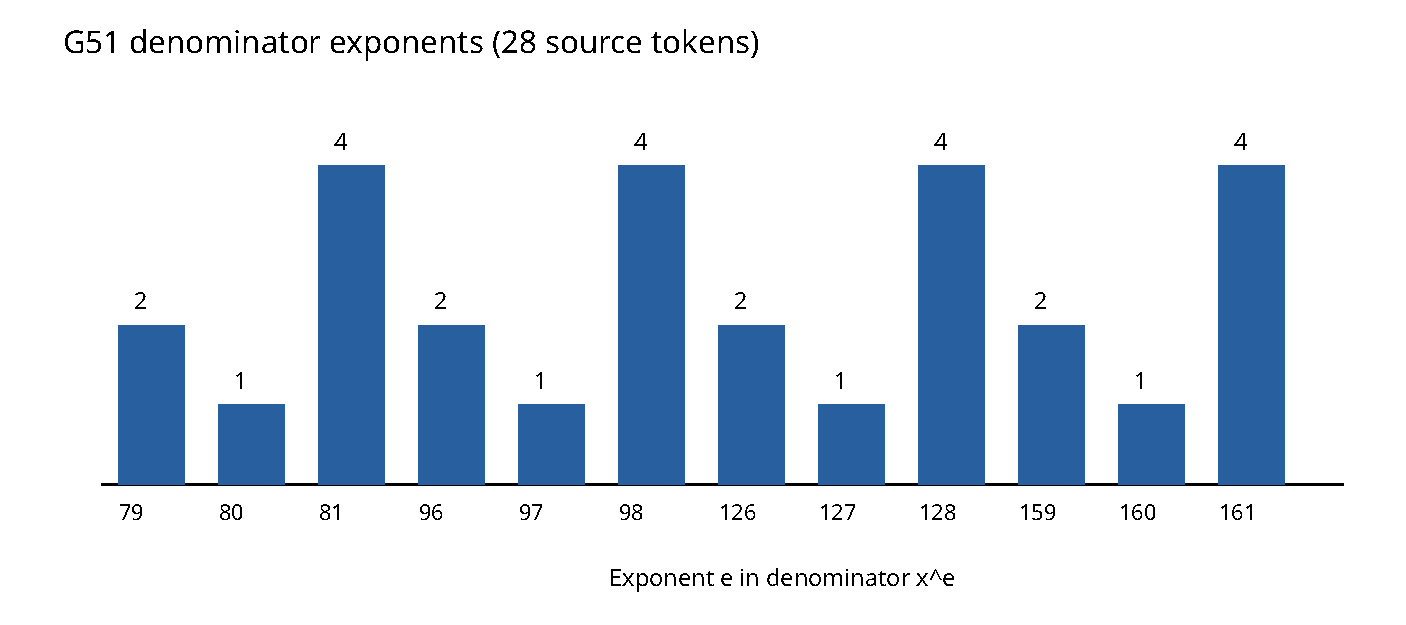
\includegraphics[width=0.95\linewidth]{diagram.pdf}
\end{center}

The next calculation is the norm of the lambda derivative resultant,
$\operatorname{Res}_y(f_{51},\operatorname{Res}_l(G_{51},\partial_lG_{51}))$,
on $D(x)$. Its zero support, together with the R97 degree-7 base-order
discriminant support and the fiber at infinity, will identify fibers for
local normalization. This report makes no normalized ramification claim.

\end{document}
